%MARCOS RIAL DOCAMPO
%Parte del documento principal TFG

%%%%%%%%%%%%%%%%
%% RESULTADOS %%
%%%%%%%%%%%%%%%%


\chapter{Resultados}
\label{cap:resultados}

\section{Análisis de separabilidad}
\subsection{Análisis visual}
Una vez introducidos los datos en R se obtienen las gráficas mostradas en la figura \ref{fig:firmas_espectrales} y el conjunto de ellas en la figura \ref{fig:ral}, de donde se pueden sacar las primeras conclusiones.\Sep

\begin{figure}
	\centering
	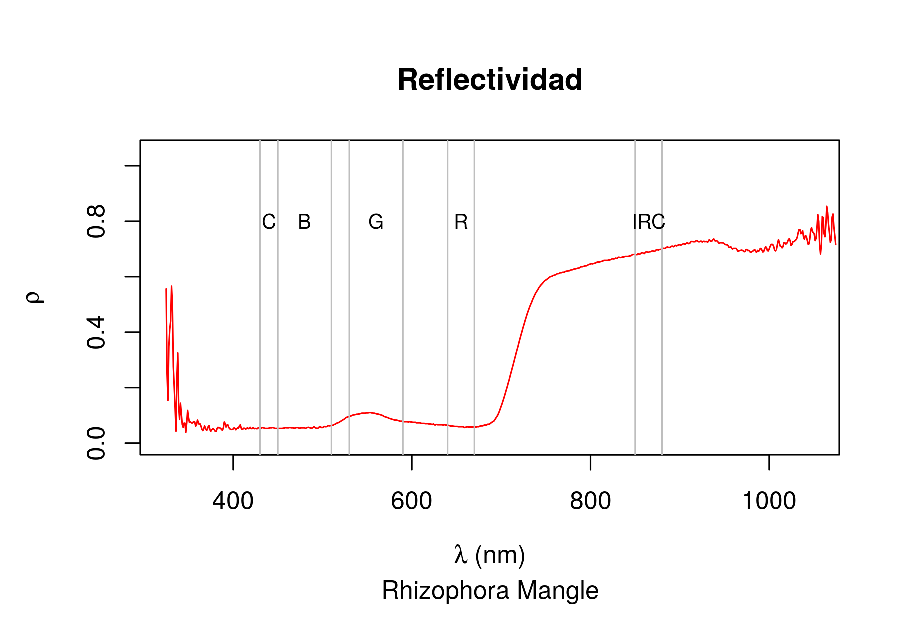
\includegraphics[width=0.8\linewidth]{./Imagenes/RM.eps}
	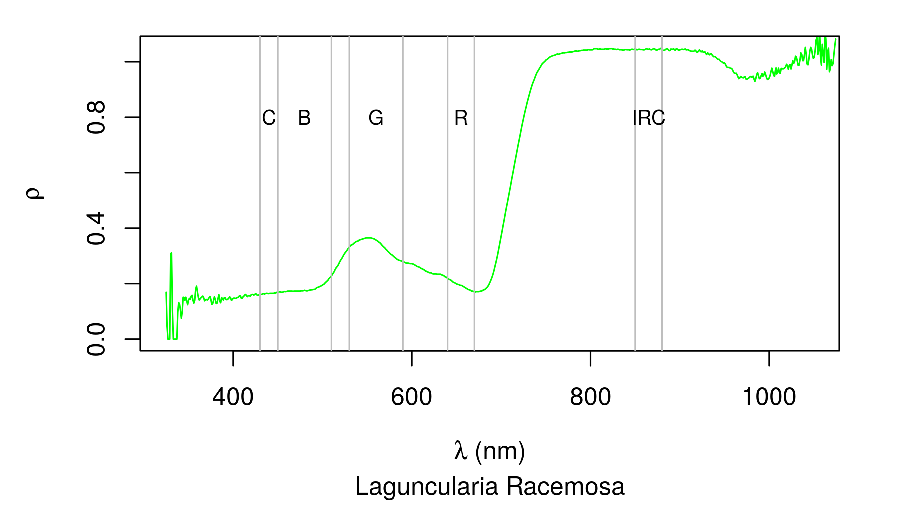
\includegraphics[width=0.8\linewidth]{./Imagenes/LR.eps}
	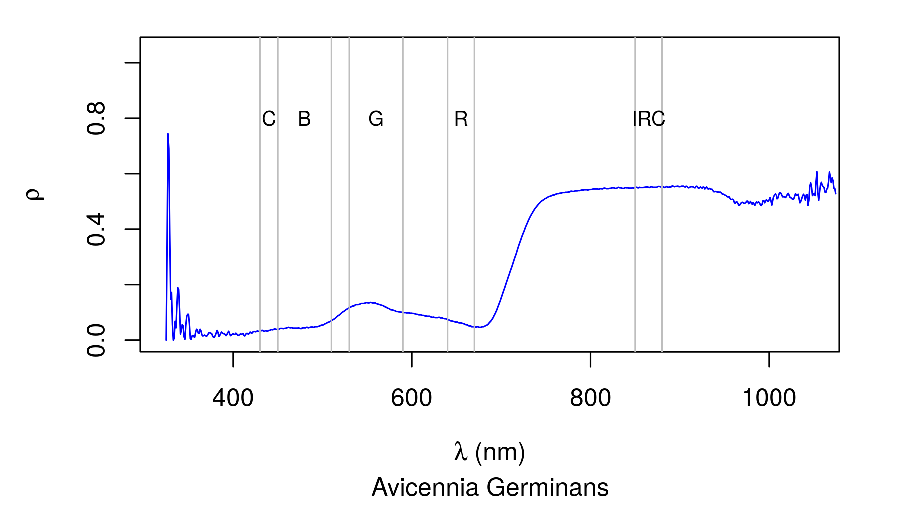
\includegraphics[width=0.8\linewidth]{./Imagenes/AG.eps}
	\captionsetup{font={footnotesize,it}}
	\caption[Firmas espectrales]{Gráficas de las firmas espectrales de las especies de mangle estudiadas. Fuente: Elaboración propia.}
	\label{fig:firmas_espectrales}
\end{figure}

\begin{figure}
	\centering
	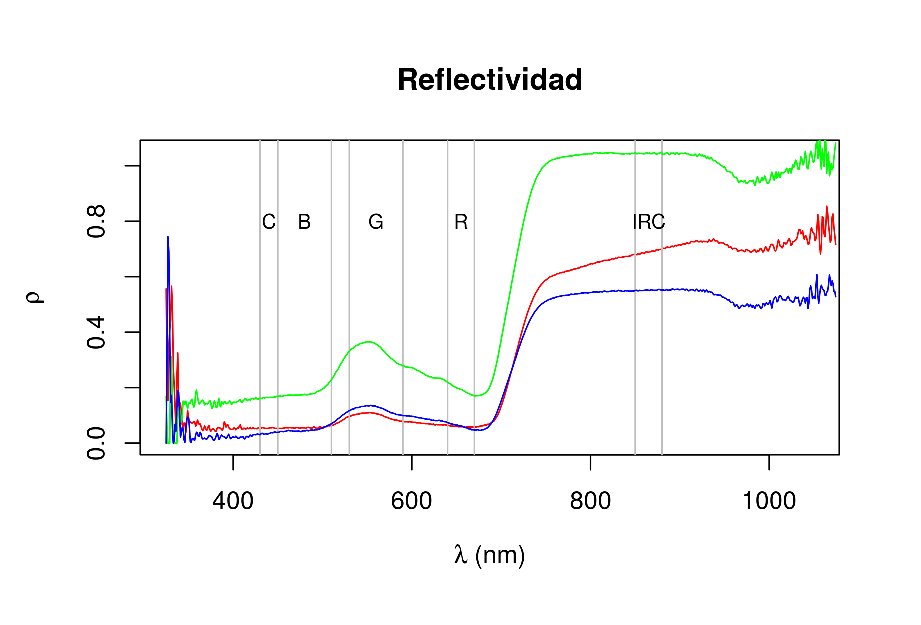
\includegraphics[width=0.8\linewidth]{./Imagenes/ral.eps}
	\captionsetup{font={footnotesize,it}}
	\caption[Firmas espectrales de las tres especies]{Gráfica conjunta de las tres firmas espectrales. Fuente: Elaboración propia.}
	\label{fig:ral}
\end{figure}

Como se aprecia en las figuras los datos presentan unas alteraciones al inicio y al final que son propias del radiómetro. Se procedió a desechar estos datos haciendo un corte de colas entre los valores 420 nm y 900 nm de longitud de onda para preservar lo máximo posible la integridad de los datos y que no afectaran a los análisis de separabilidad. El número de observaciones se reduciría a 481 por las 751 originales. Las gráficas resultantes son las mostradas en las figuras \ref{fig:firmas_espectrales_corte} y \ref{fig:ral_corte}.\Sep

\begin{figure}
	\centering
	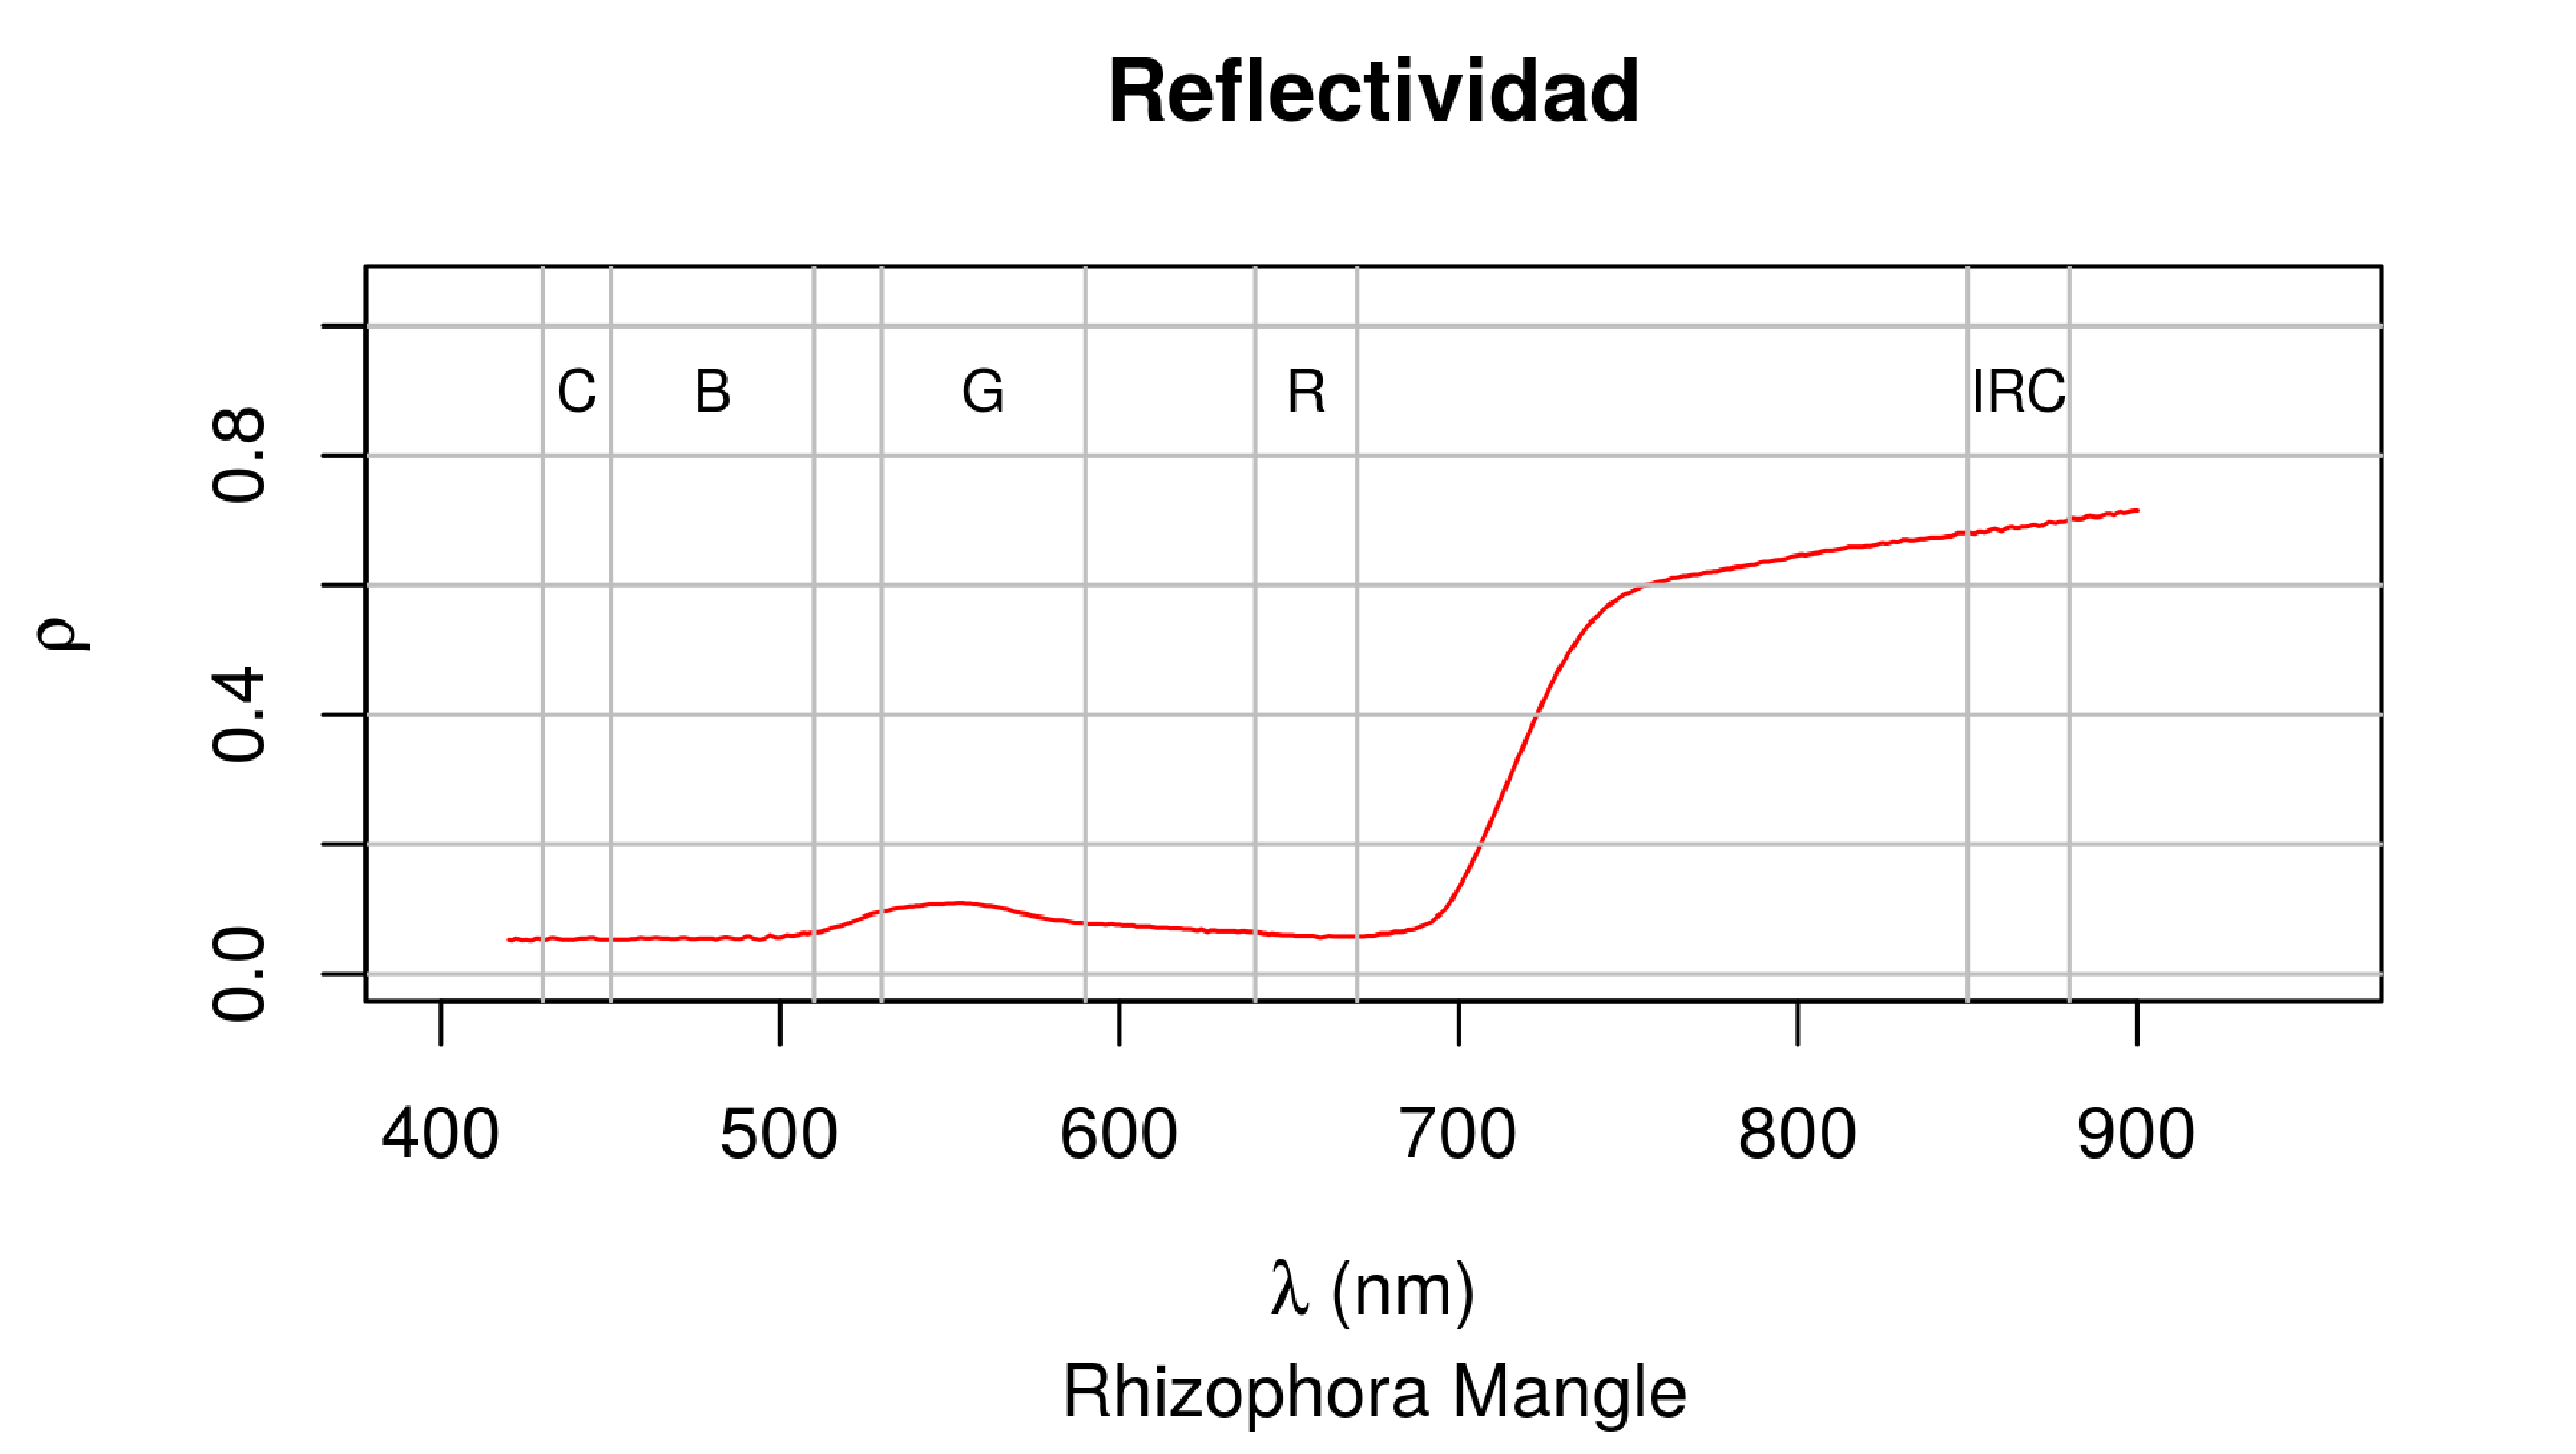
\includegraphics[width=0.8\linewidth]{./Imagenes/RMcorte.eps}
	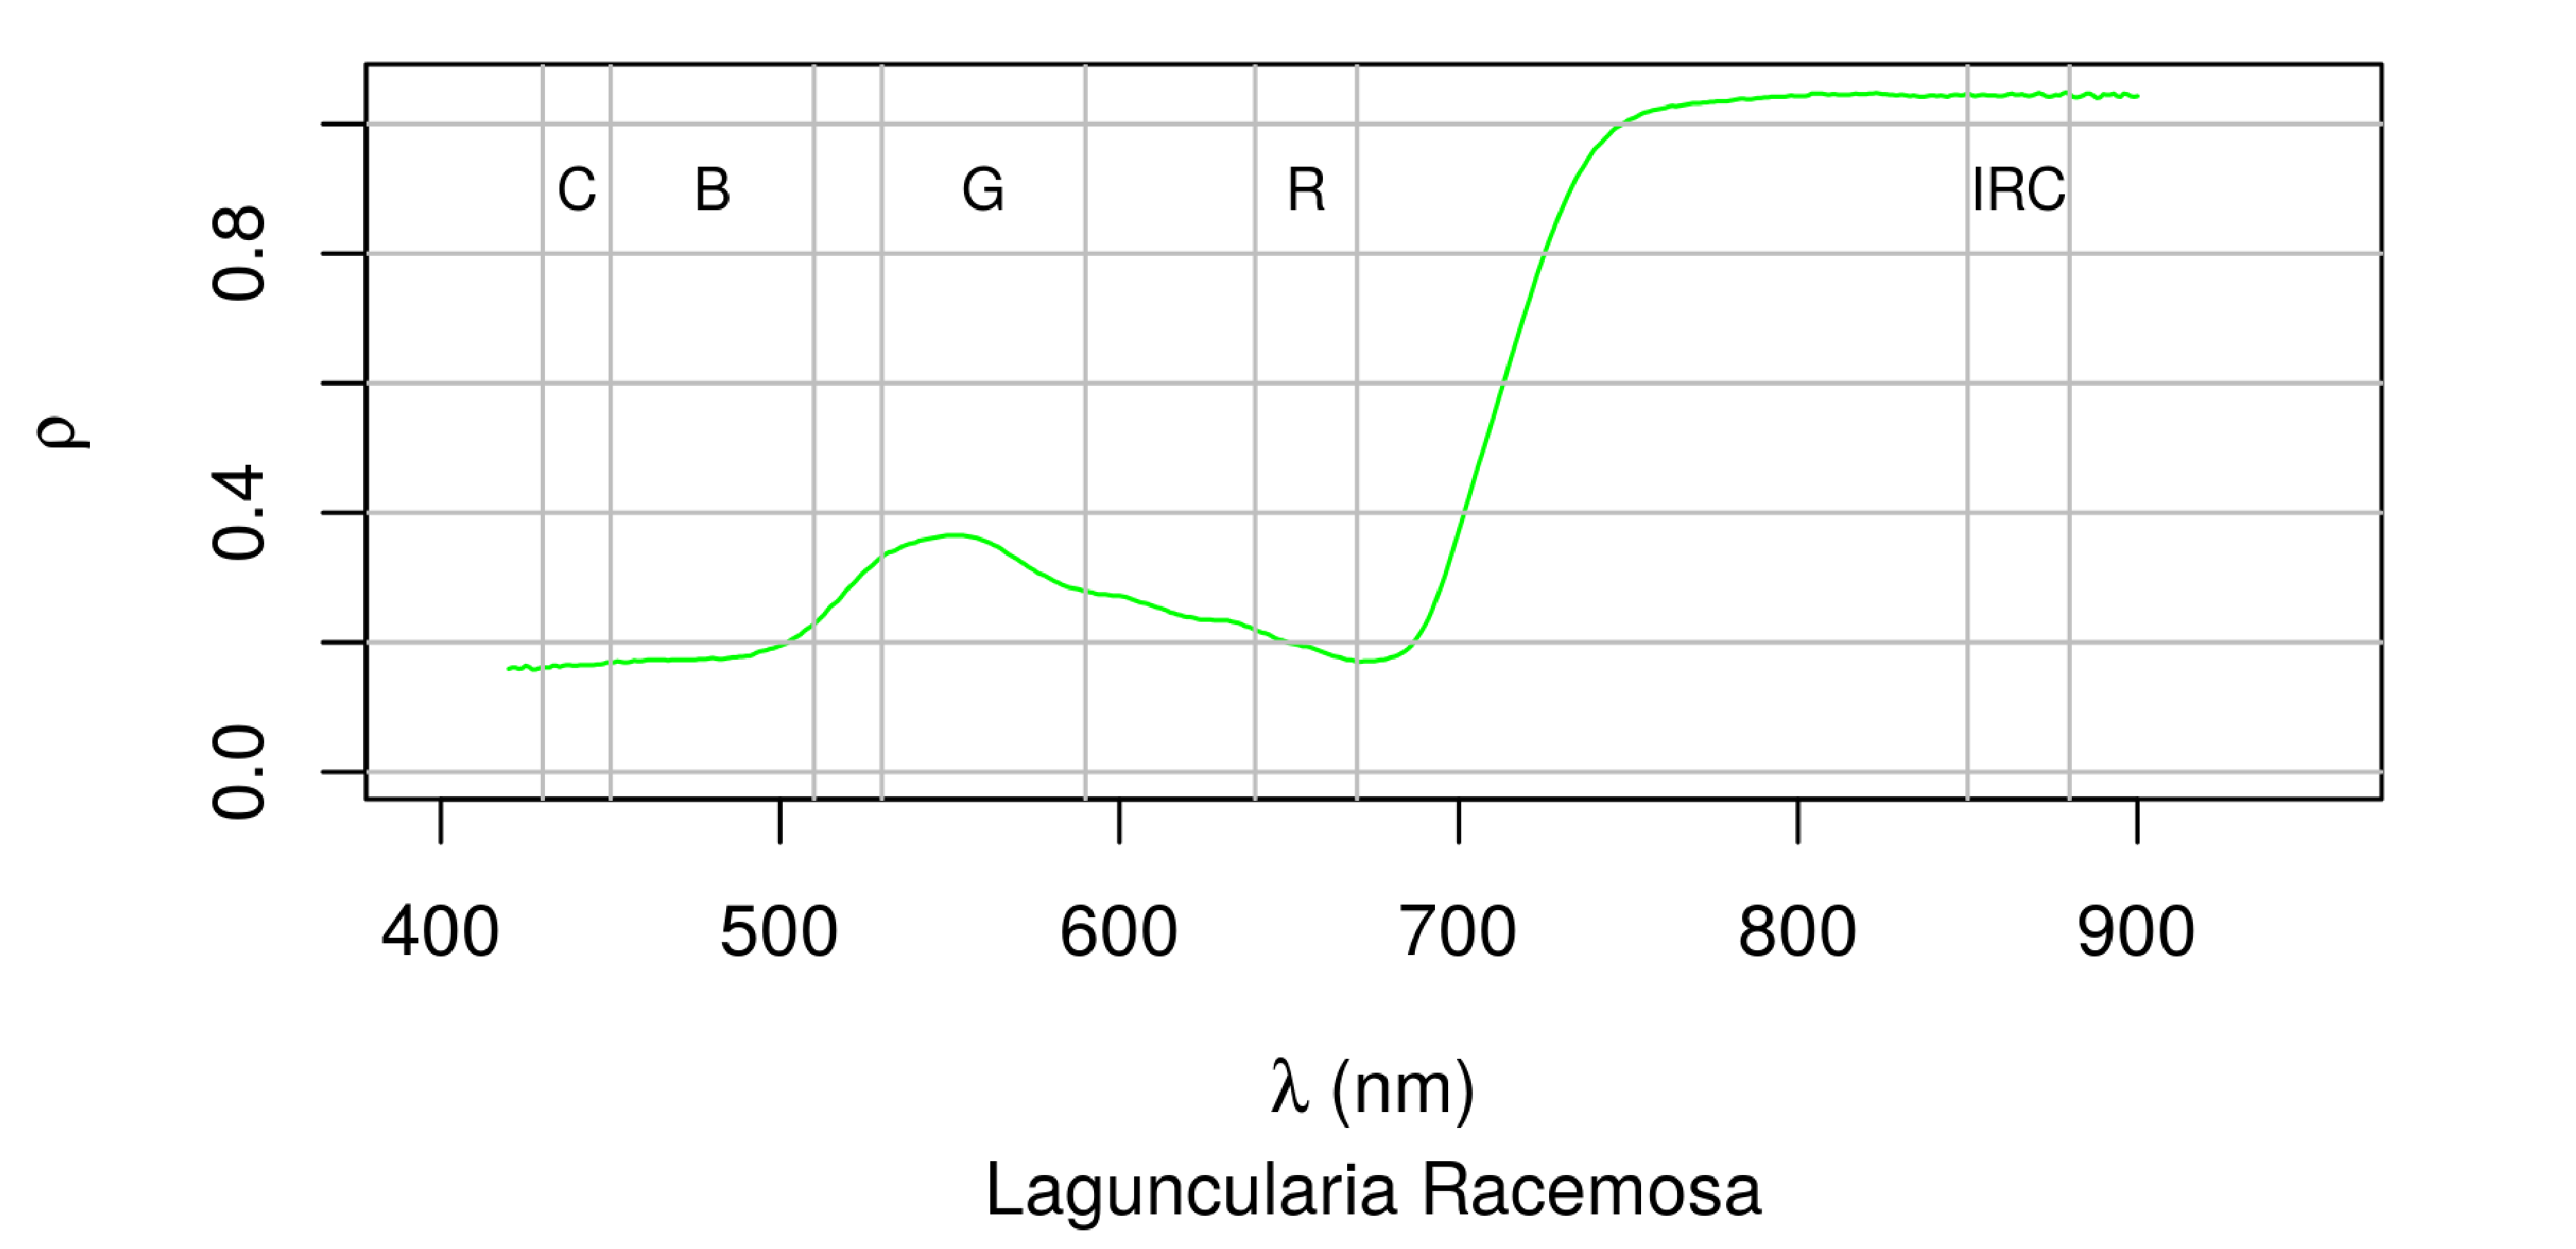
\includegraphics[width=0.8\linewidth]{./Imagenes/LRcorte.eps}
	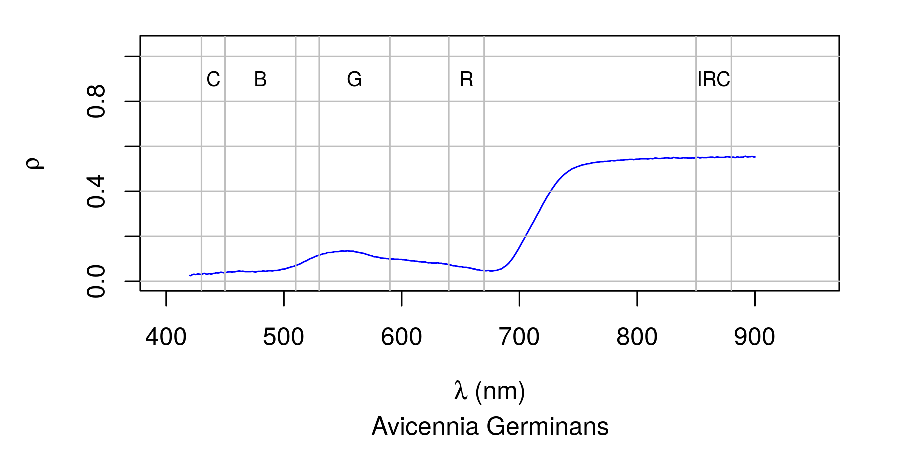
\includegraphics[width=0.8\linewidth]{./Imagenes/AGcorte.eps}
	\captionsetup{font={footnotesize,it}}
	\caption[Firmas espectrales cortadas]{Gráficas de las firmas espectrales de las especies de mangle estudiadas una vez realizado el corte de los datos. Fuente: Elaboración propia.}
	\label{fig:firmas_espectrales_corte}
\end{figure}

\begin{figure}
	\centering
	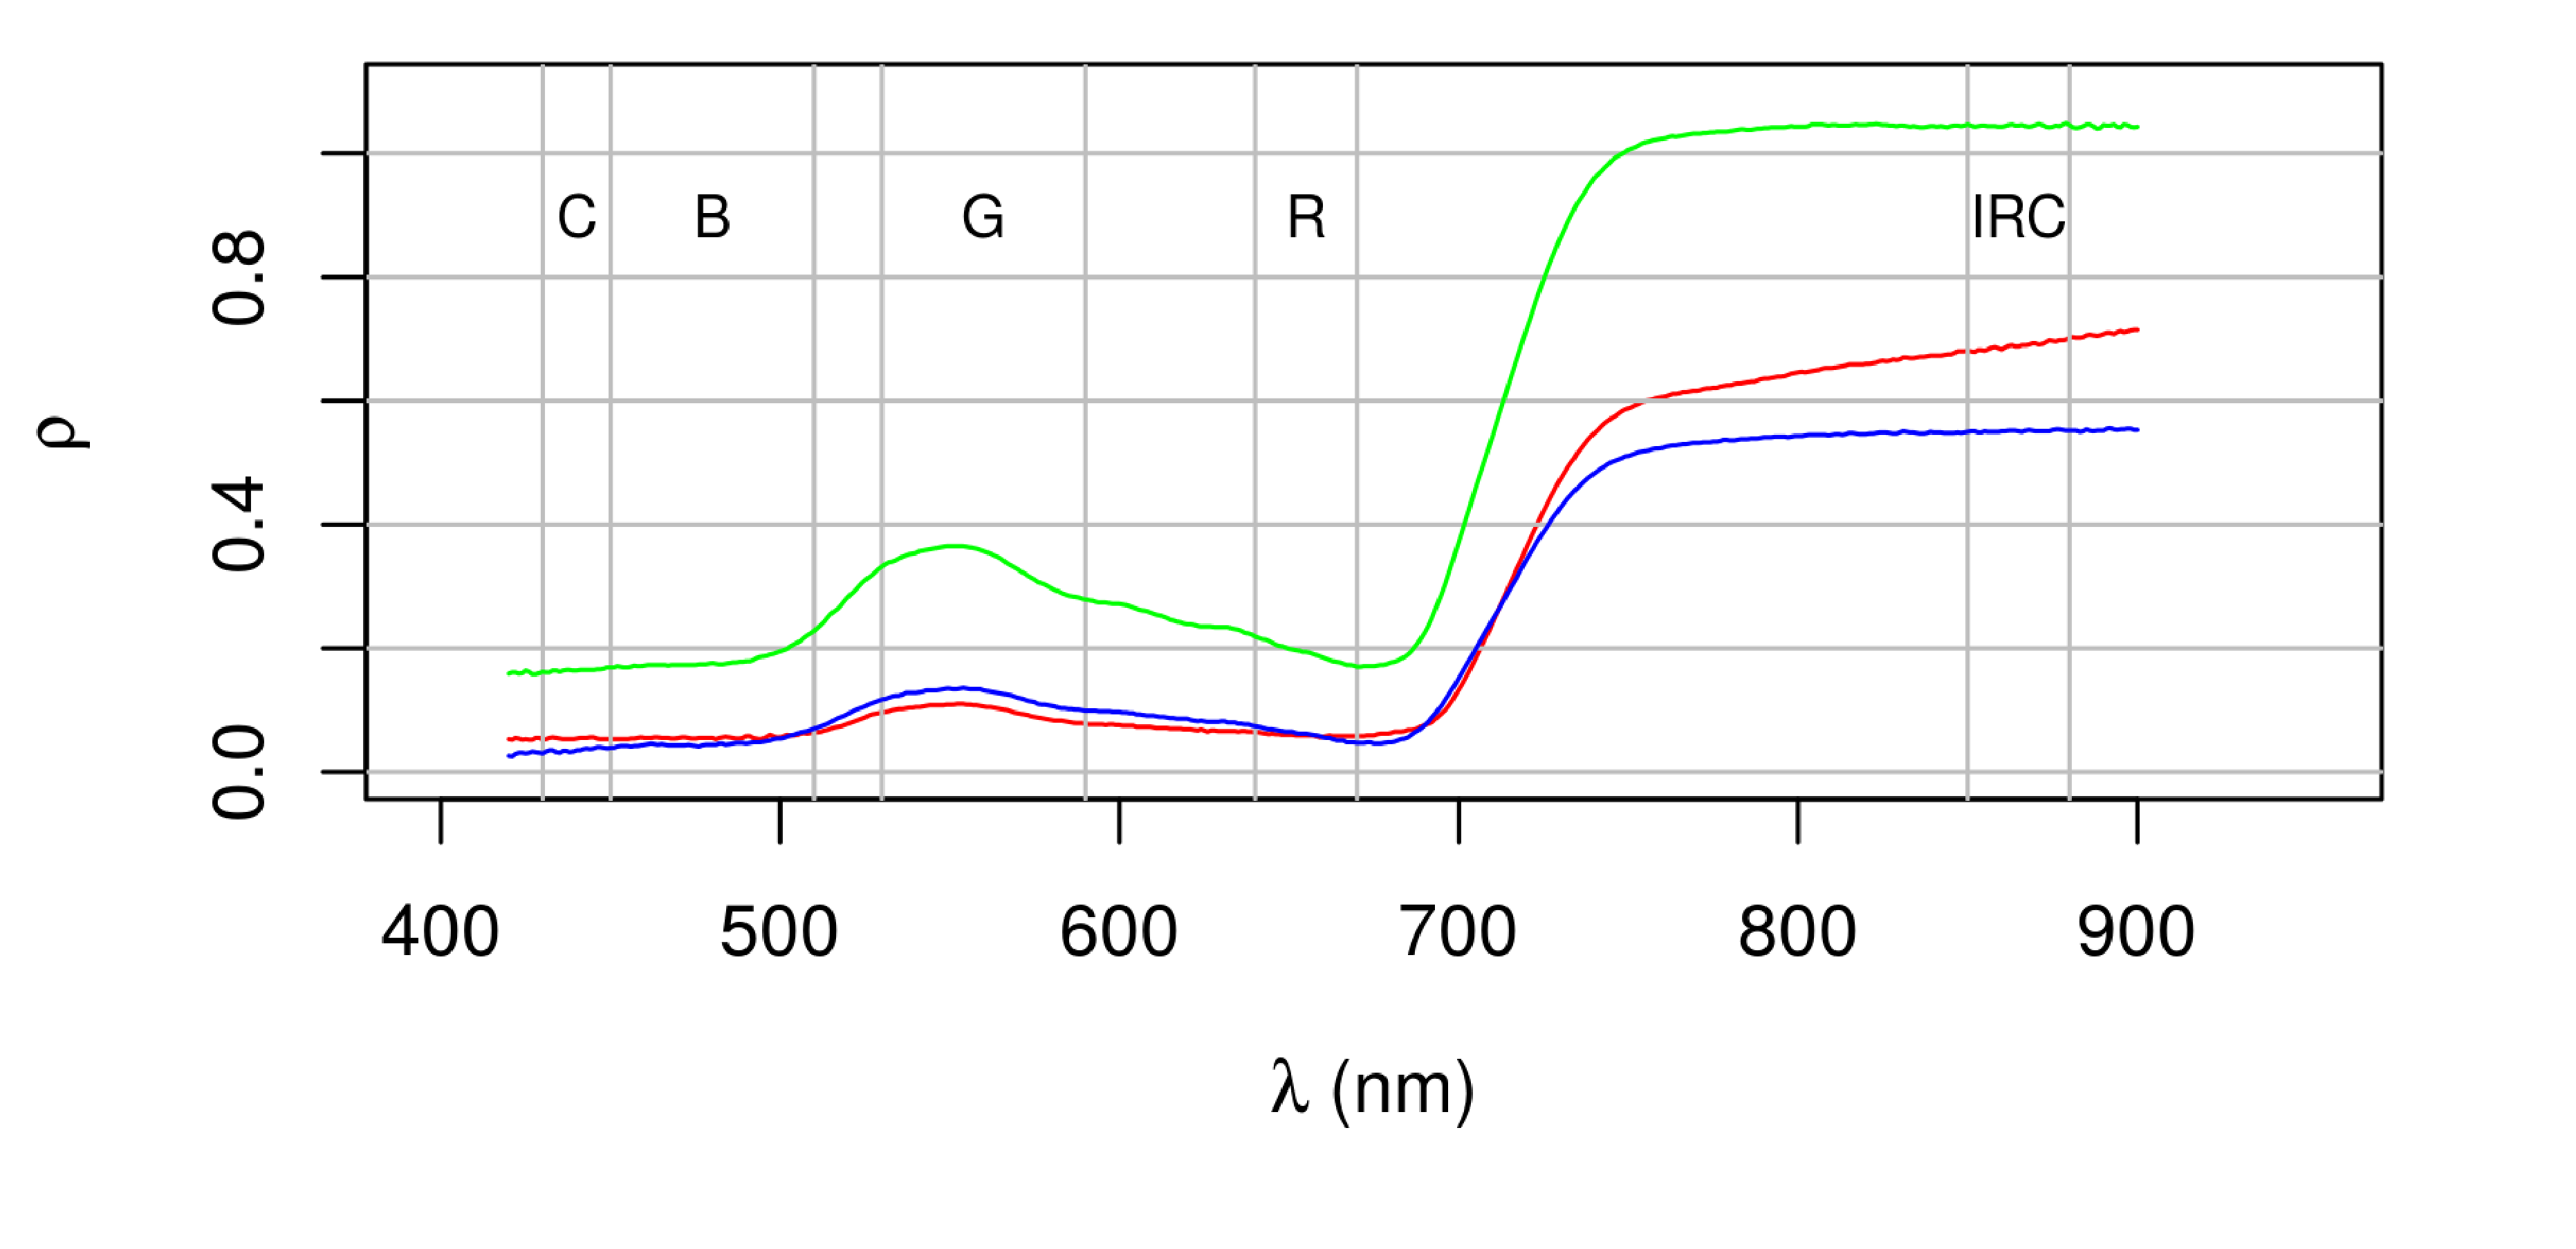
\includegraphics[width=0.8\linewidth]{./Imagenes/ralcorte.eps}
	\captionsetup{font={footnotesize,it}}
	\caption[Firmas espectrales cortadas de las tres especies]{Gráfica conjunta de las tres firmas espectrales una vez realizado el corte de los datos. Fuente: Elaboración propia.}
	\label{fig:ral_corte}
\end{figure}

Las tres especies tienen un máximo local en la banda correspondiente al verde (G), típica de las especies vegetales, así como otro máximo de mayor valor, correspondientes al intervalo de longitud de onda ($\lambda$) en el que está incluida la banda del \ac{IRC}. Este último máximo también es característico de la vegetación e indicaría su grado de salud.\Sep

Por lo tanto el primer vistazo a las gráficas es el esperado, siendo lo más preocupante el aparente parecido entre las especies R. mangle y A. germinans, que solo se diferencian en el valor del \ac{IRC}.\Sep

En el cuadro siguiente se pueden apreciar los valores medios de cada especie para cada banda de Landsat 8

\begin{table}[ht]
	\centering
	\caption[Valores medios en las bandas Landsat]{Valores medios ara cada banda Landsat. Fuente: Elaboración propia.}
	\begin{tabular}{@{}cccccc@{}}
	\toprule[0.4mm]
	Especie & Banda 1 (C) & Banda 2 (B) & Banda 3 (G) & Banda 4 (R) & Banda 5 (IRC) \\
	\midrule
	\textit{R. mangle}	& 0.0540 & 0.0561 & 0.0980 & 0.0595 & 0.6895 \\
	\textit{L. racemosa} & 0.1647 & 0.1821 & 0.3345 & 0.1930 & 1.0445 \\
	\textit{A. germinans} & 0.0355 & 0.0479 & 0.1218 & 0.0604 & 0.5513 \\
	\bottomrule[0.4mm]
	\end{tabular}
\end{table}

%\section{Aplicación de los análisis}
\subsection{Índice de Acuerdo Espectral}
Una vez aplicando el script con la función de \ac{IAE} creado en R (figura \ref{fig:IAE}) ya se aprecia que el resultado no es muy bueno, aunque esperado, siendo las diferencias casi inapreciables como se ve en la tabla \ref{tab:Valores_IAE} y en los gráficos de la figura \ref{fig:CB}, donde se aprecia mejor la poca diferencia espectral existente.\Sep

\begin{table}[ht]
	\centering
	\caption[Valores de IAE]{Valores de \ac{IAE} para cada par de especies de mangle. Fuente: Elaboración propia.}
	\begin{tabular}{@{}cccc@{}}
	\toprule
	& \textit{R. mangle} & \textit{L. racemosa} & \textit{A. germinans} \\
	\textit{R. mangle} & --- & 0.0083 & 0.0062 \\
	\textit{L. racemosa} & 0.0083 & --- & 0.0021 \\
	\textit{A. germinans} & 0.0062 & 0.0021 & --- \\
	\bottomrule[0.4mm]
	\end{tabular}
	\label{tab:Valores_IAE}
\end{table}

Las diferencias en este método son bajas debido a que se trata de tres especies que, aunque no sean de la misma familia, si son vegetales y coexisten formando asociación en el mismo ecosistema. De haber estudiado la diferencia entre especie vegetal, suelo y agua por ejemplo, las diferencias habrían sido más notables debido a la diferencia de valor medio de la respuesta espectral. En este caso, el valor medio de las tres especies sería el mostrado en la tabla siguiente:

\begin{table}[ht]
	\centering
	\caption[Valores medios de la respuesta espectral]{Valor medio de la respuesta espectral para cada especie.}
	\begin{tabular}{@{}ccc@{}}
	\toprule[0.4mm]
	Especie & $\rho$ media & Corte en $\lambda$ (nm)\\
	\midrule
	\textit{R. mangle} & 0.2897692 & 714	\\
	\textit{L. racemosa} & 0.5424927 & 710\\
	\textit{A. germinans} & 0.2530166 & 711\\
	\bottomrule
	\end{tabular}
	\label{tab:mediaIAE}
\end{table}

El corte en $\lambda$ que se menciona en el cuadro \ref{tab:mediaIAE} se refiere al valor de longitud de onda a partir del cual la reflectancia es mayor a la media y por tanto se provoca una cambio en el valor binario de 0 a 1 donde, de tener un mayor rango de longitud de onda observada habría más de un cambio. Se observan unos valores similares de $\lambda$ para las tres especies, pero donde sí se notan diferencias son en el valor medio de la reflectancia, siendo el de la \textit{L. racemosa} notablemente superior al de las otras dos especies.

\begin{figure}
	\centering
	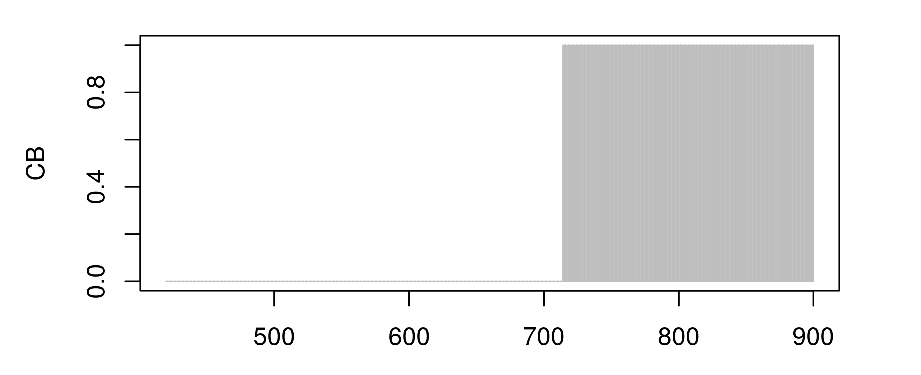
\includegraphics[width=0.8\linewidth]{./Imagenes/IAE_RM.eps}
	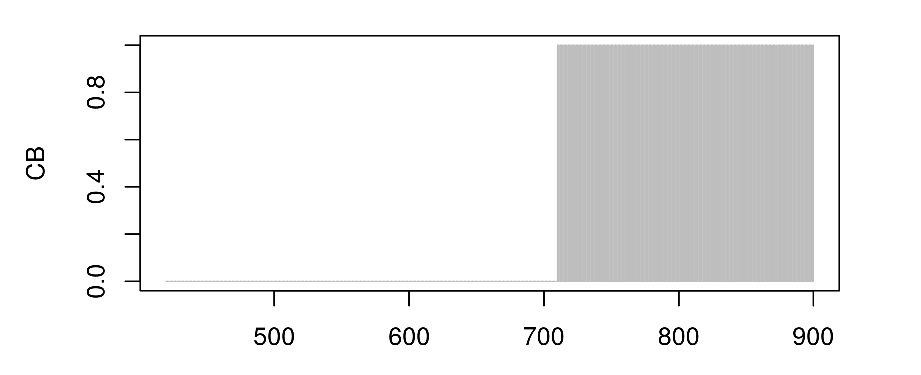
\includegraphics[width=0.8\linewidth]{./Imagenes/IAE_LR.eps}
	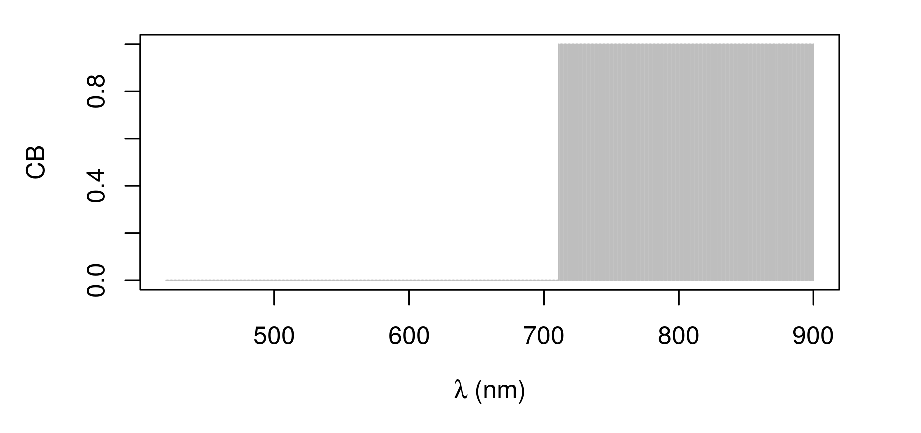
\includegraphics[width=0.8\linewidth]{./Imagenes/IAE_AG.eps}
	\captionsetup{font={footnotesize,it}}
	\caption[Gráficas de combinación binaria]{Gráficas de combinación binaria de las tres especies de mangle, por orden \textit{Rhizophora mangle}, \textit{Laguncularia racemosa} y \textit{Avicennia germinans}. Fuente: Elaboración propia.}
	\label{fig:CB}
\end{figure}

\subsection{Continuum Removal}
En la gráfica de la figura \ref{fig:GraficaCR} se pueden observar las diferencias entre las tres especies que nos indica este tipo de análisis. Son tres los aspectos de esta gráfica a analizar: la profundidad y anchura de las partes convexas y la posición de los puntos mínimos. En gris la gráfica de reflectividad de cada especie.\Sep

\begin{figure}
	\centering
	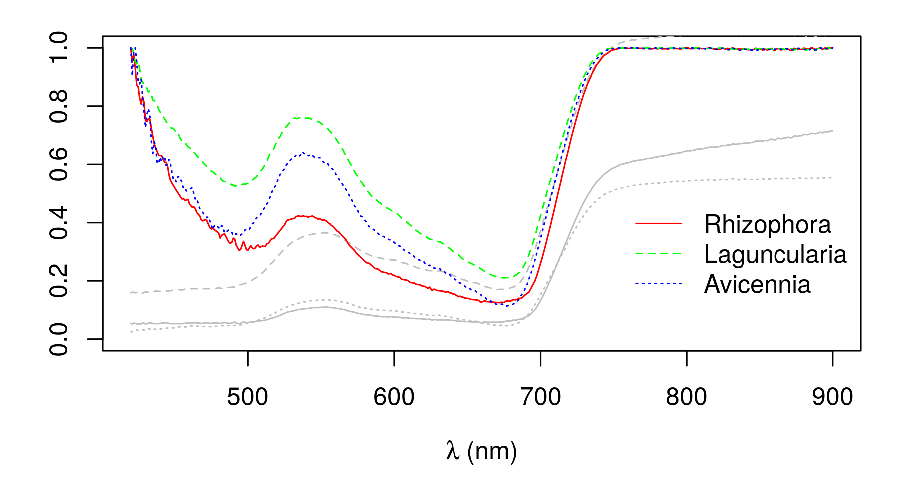
\includegraphics[width=0.8\linewidth]{./Imagenes/ContinuumR2.eps}
	\captionsetup{font={footnotesize,it}}
	\caption[Gráfica de Continuum Removal]{Gráfica de continuum removal para las tres especies de mangle. Fuente: Elaboración propia.}
	\label{fig:GraficaCR}
\end{figure}

En cuanto a la profundidad se observa una clara absorción en torno a los 490 nm y los 680 nm de las tres especies. En el caso de la \textit{A. germinans} esta absorción es más acusada en ambos puntos. \textit{R. mangle} y \textit{L. racemosa} muestran un comportamiento similar en la primera zona mientras que en la segunda la \textit{L. racemosa} no muestra la absorción de la \textit{R. mangle}.\Sep

En cuanto a la anchura lo más llamativo es la amplitud de los valores de la \textit{R. mangle} en torno a los valores centrales de la observación.

\subsection{Clasificación angular}
Una vez aplicado el script de R de la función de clasificación angular (figura \ref{fig:AE}), los valores son los de la siguiente tabla:

\begin{table}[ht]
	\centering
	\caption[Valores de Ángulo Espectral]{Valores del Ángulo Espectral en radianes. Ángulo centesimal entre paréntesis.}
	\begin{tabular}{@{}cccc@{}}
	\toprule[0.4mm]
	& \textit{R. mangle} & \textit{L. racemosa} & \textit{A. germinans} \\
	\textit{R. mangle} & --- & 0.1651 (10.5085) & 0.0752 (4.7874) \\
	\textit{L. racemosa} & 0.1651 (10.5085) & --- & 0.1062 (6.7584) \\
	\textit{A. germinans} & 0.0752 (4.7874) & 0.1062 (6.7584) & --- \\
	\bottomrule[0.4mm]
	\end{tabular}
\end{table}

Se puede observar una mayor separabilidad entre \textit{R. mangle} y \textit{L. racemosa}, siendo menor en las otras combinaciones.

\section{Comprobación}
Debemos saber si los datos de reflectividad de las especies de mangle se adaptan a los datos de las imágenes raster de Landsat 8 que se han corregido. Para ello tomamos la serie de puntos en los que se conoce la existencia de bosque de mangle (cuadro \ref{tab:puntos}). Se creará en GRASS una capa vectorial con estos puntos a las que se le añadirán los valores raster de reflectividad de cada banda. Los pasos a seguir fueron los siguientes:

\begin{itemize}
	\item Creación de una capa vectorial en blanco de nombre ``puntos'' y añadirla al árbol de capas. En esta capa se digitalizarán un total de 10 puntos en los que se supone la existencia de bosque de mangle.
	\item Crear una base de datos asociada a la capa con \textit{v.db.addtable} asignando nuevos campos: ``x'' e ``y'' de tipo ``double'' que se actualizarán con las coordenadas de los puntos. También se añadirán a la tabla columnas para alojar el valor de los datos de cada una de las bandas en cada punto nombradas como B1, B2, B3, B4 y B5 de tipo ``double''.
	\item Actualización de los campos de coordenadas mediante el comando \textit{v.to.db} como se muestra en la figura \ref{fig:v.to.db} donde \textit{map} designa el vectorial que tiene la tabla asociada, \textit{option} indica que queremos actualizar coordenadas y \textit{columns} son los nombres de las columnas de coordenadas de nuestra tabla.
	
\begin{figure}[ht]
\centering
\begin{boxedverbatim}
	v.to.db map=puntos@TFG option=coor columns=x,y
\end{boxedverbatim}
\captionsetup{font={footnotesize,it}}
\caption[Actualización de coordenadas]{Actualización del campo coordenadas en GRASS con el comando \textit{v.to.db}.}
\label{fig:v.to.db}
\end{figure}	
	
	\item Actualización de los campos de datos del raster mediante el comando \textit{v.what.rast} como se muestra en la figura \ref{fig:v.what.rast} donde \textit{vector} indica cual es el vectorial que deseamos actualizar, \textit{raster} es el raster del que se tomarán los datos y \textit{column} el nombre del campo a actualizar.
\end{itemize}

\begin{figure}[ht]
\centering
\begin{boxedverbatim}
	v.what.rast vector=puntos@TFG raster=L8GF_SRFB1@TFG column=B1
\end{boxedverbatim}
\captionsetup{font={footnotesize,it}}
\caption[Actualización de los datos raster]{Actualización de los campos de datos raster en GRASS con el comando \textit{v.what.rast}.}
\label{fig:v.what.rast}
\end{figure}

Los gráficos extraídos de la base de datos de la capa ``puntos'' de GRASS son las mostradas en las figuras \ref{fig:puntos_comprob} y \ref{fig:puntos_comprob2}. En ellos se muestra el valor que devuelve el raster de cada banda en cada punto. Se muestran los valores en el cuadro \ref{tab:tabla_puntos}.\Sep

\begin{table}[ht]
	\centering
	\caption[Base de datos de puntos de comprobación]{Base de datos asociada a la capa vectorial ``puntos''.}
	\begin{tabular}{@{}rccccccc@{}}
	\toprule[0.4mm]
	cat & x & y & B1 & B2 & B3 & B4 & B5\\
	\midrule
	1 & 415596 & 1483332 & 87 & 106 & 271 & 130 & 3309\\
	2 & 414143 & 1481608 & 98 & 116 & 289 & 135 & 3322\\
	3 & 417524 & 1481222 & 101 & 123 & 304 & 159 & 2977\\
	4 & 420792 & 1477569 & 182 & 214 & 379 & 314 & 1793\\
	5 & 426578 & 1480632 & 158 & 202 & 386 & 313 & 1957\\
	6 & 433952 & 1483185 & 86 & 100 & 244 & 122 & 3002\\
	7 & 440238 & 1477444 & 129 & 157 & 350 & 232 & 2320\\
	8 & 450698 & 1475867 & 123 & 154 & 389 & 220 & 2847\\
	9 & 447771 & 1466825 & 100 & 124 & 254 & 154 & 2368\\
	10 & 450448 & 1464351 & 102 & 119 & 300 & 159 & 2934\\
	\bottomrule[0.4mm]
	\end{tabular}
	\label{tab:tabla_puntos}
\end{table}

\begin{figure}
\centering
\subfloat[Datos punto 1]{
	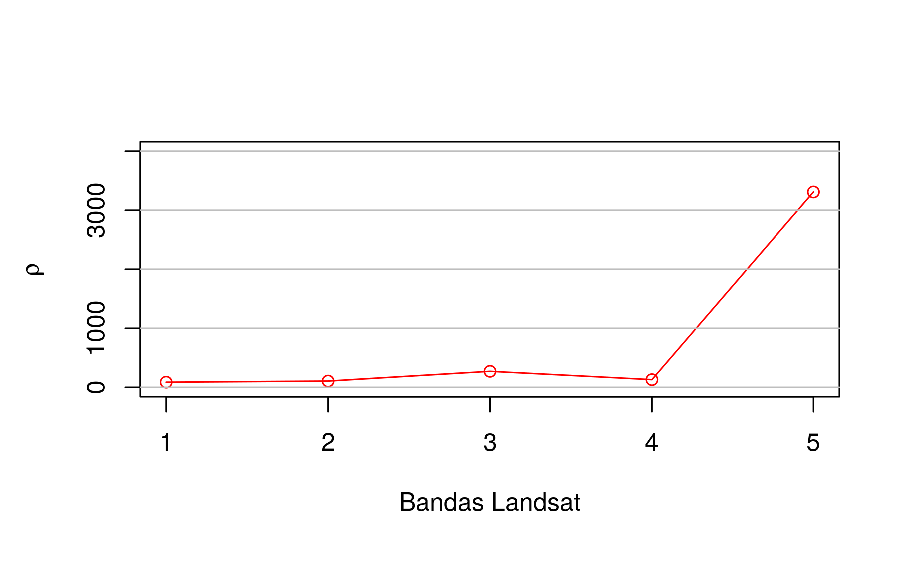
\includegraphics[width=0.45\linewidth]{./Imagenes/punto1.eps}}
\subfloat[Datos punto 2]{
	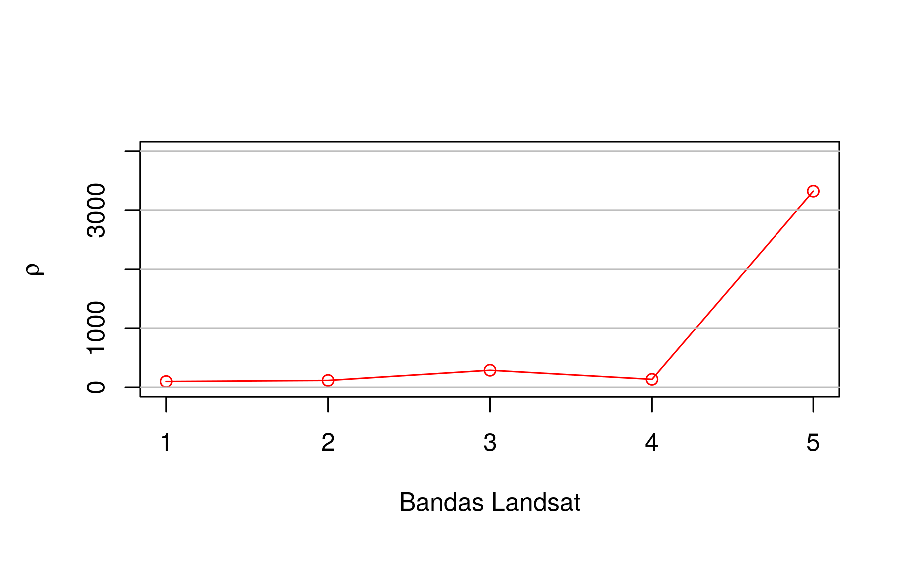
\includegraphics[width=0.45\linewidth]{./Imagenes/punto2.eps}}\\
\subfloat[Datos punto 3]{
	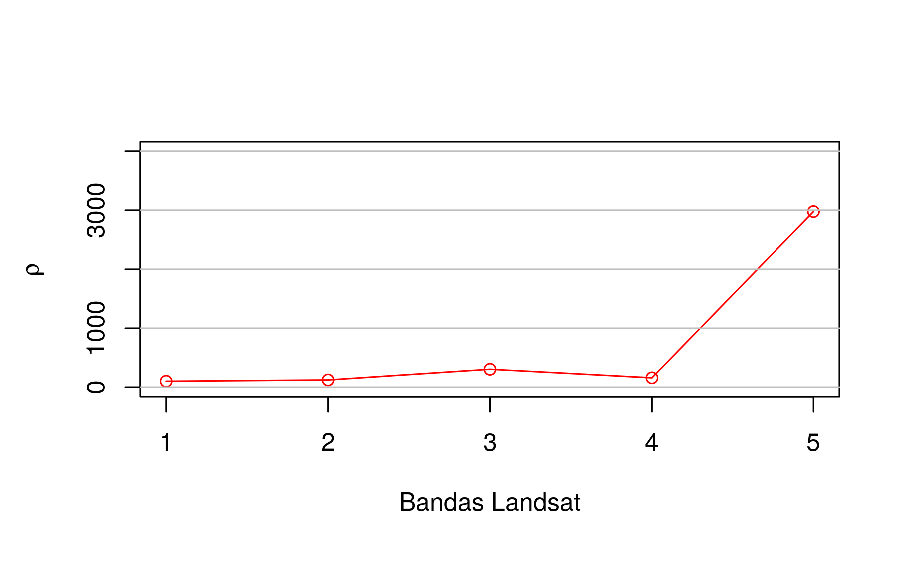
\includegraphics[width=0.45\linewidth]{./Imagenes/punto3.eps}}
\subfloat[Datos punto 4]{
	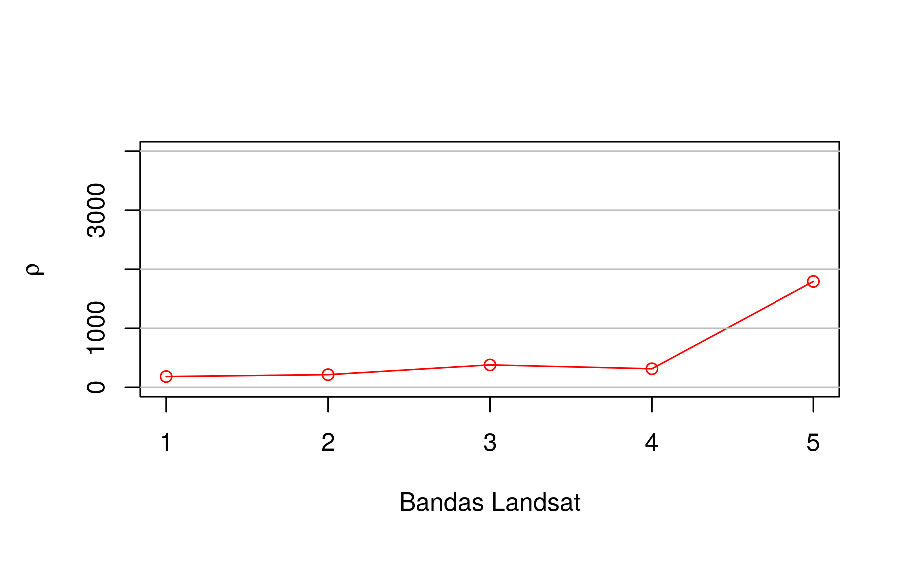
\includegraphics[width=0.45\linewidth]{./Imagenes/punto4.eps}}\\
\subfloat[Datos punto 5]{
	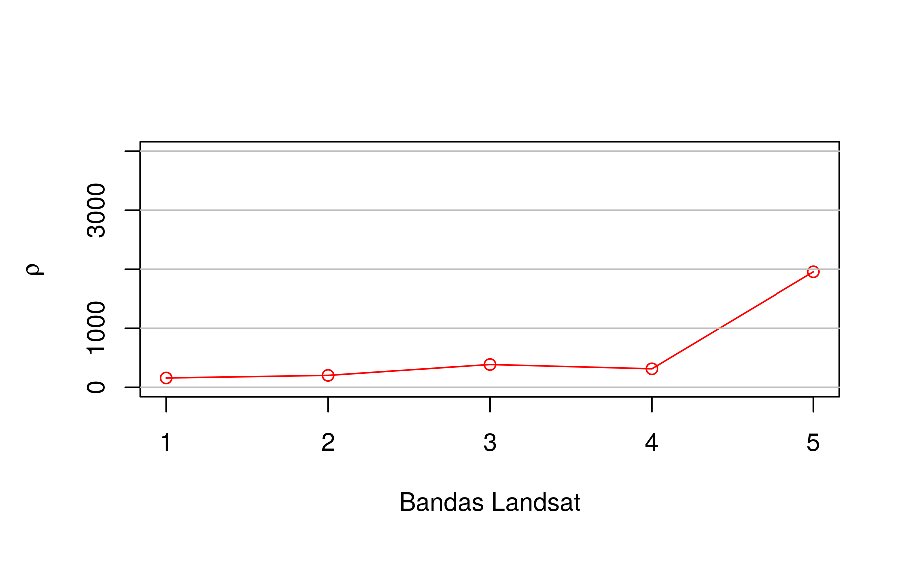
\includegraphics[width=0.45\linewidth]{./Imagenes/punto5.eps}}
\subfloat[Datos punto 6]{
	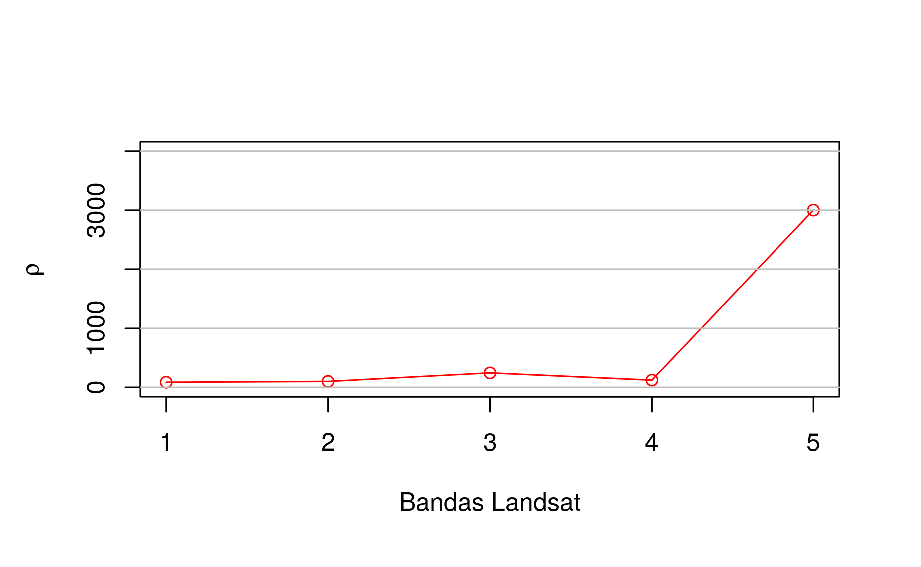
\includegraphics[width=0.45\linewidth]{./Imagenes/punto6.eps}}\\
\subfloat[Datos punto 7]{
	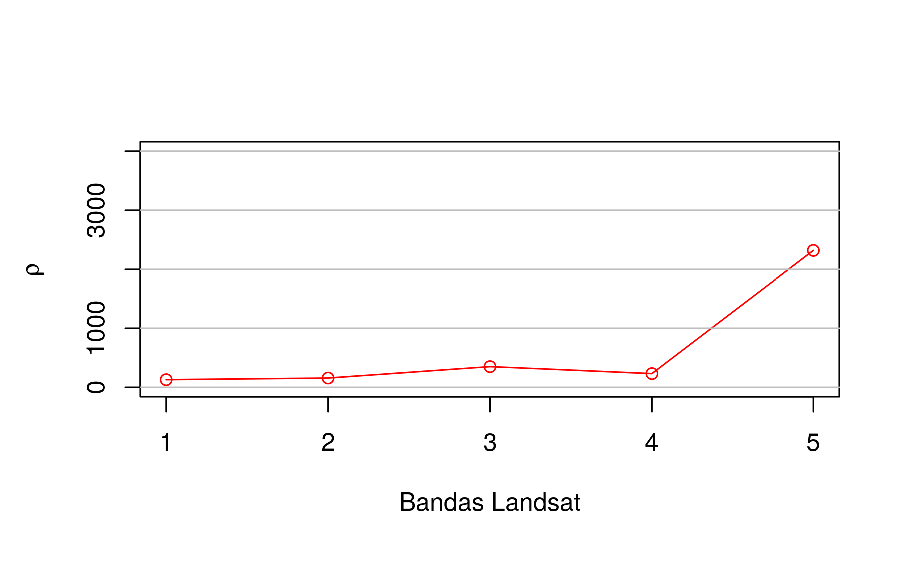
\includegraphics[width=0.45\linewidth]{./Imagenes/punto7.eps}}
\subfloat[Datos punto 8]{
	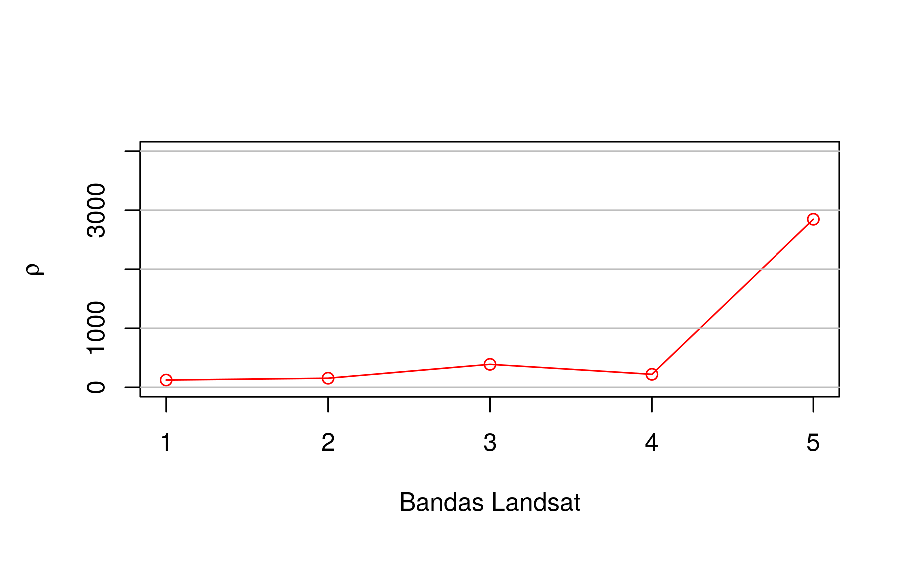
\includegraphics[width=0.45\linewidth]{./Imagenes/punto8.eps}}
\captionsetup{font={footnotesize,it}}
\caption[Gráficas puntos de comprobación]{Gráficas de los puntos de comprobación tomados. Fuente: Elaboración propia.}
\label{fig:puntos_comprob}	
\end{figure}

\begin{figure}
\centering
\subfloat[Datos punto 9]{
	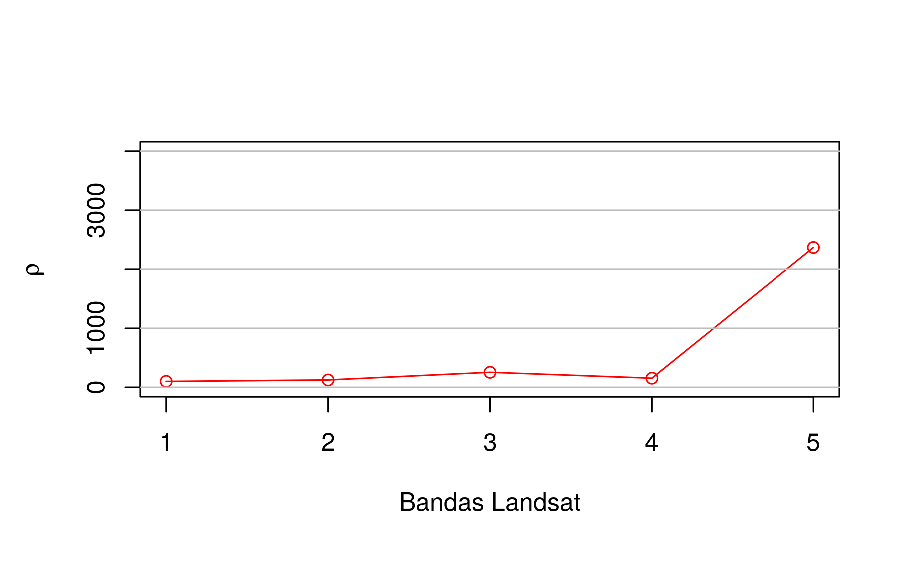
\includegraphics[width=0.45\linewidth]{./Imagenes/punto9.eps}}
\subfloat[Datos punto 10]{
	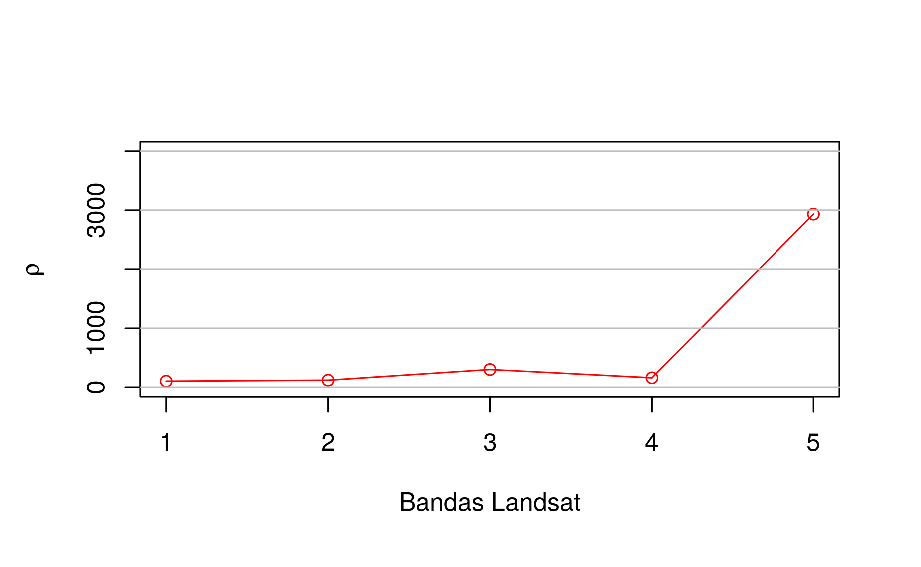
\includegraphics[width=0.45\linewidth]{./Imagenes/punto10.eps}}
\captionsetup{font={footnotesize,it}}
\caption[Gráficas puntos de comprobación]{Gráficas de los puntos de comprobación tomados. Fuente: Elaboración propia.}
\label{fig:puntos_comprob2}
\end{figure}

Puede observarse que los valores extraídos son valores enteros debido a que la corrección utilizada en las imágenes \ac{PL8SR} los valores vienen presentados con un factor de escala 0.0001 \citep{USGS2015}.